\beginsong{Tandaradei}[
    wuw={Text und Musik nach alten Vorlagen von umba (Jürgen W. Diener)}, 
    jahr={1986}, 
    pfii={26}, 
    pfiii={70}, 
    bo={230}, 
    siru={161}, 
    index={Mädchen, Männer, Meister wert},
]

\beginverse
\endverse
\centering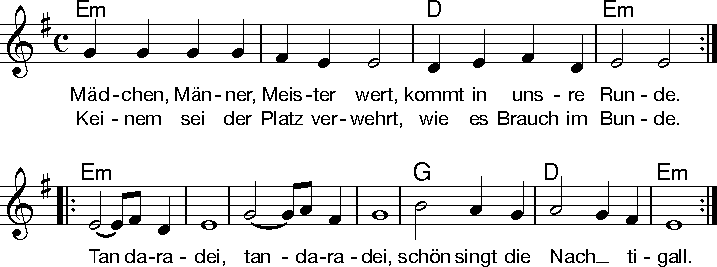
\includegraphics[width=1\textwidth]{Noten/Lied083.pdf}

\beginverse
\[Em]Von der Runde frohen Schall 
\[D]hallt das Lager \[Em]wieder,
\[Em]und es singt Frau Nachtigall 
\[D]ihre schönsten \[Em]Lieder.
\endverse

\beginchorus
\[Em]Tan-da-ra-dei, tan-da-ra-dei, \[G]schön singt die \[D]Nachti\[Em]gall.
\endchorus

\beginverse
^Ist auch dieses Liedes Schall ^allzu rasch ver^klungen,
^Sommerlust ist überall, ^freuet euch, ihr ^Jungen.
\endverse\renewcommand{\everychorus}{\textnote{\bf Refrain (wdh.)}}
\beginchorus
\endchorus

\endsong

\beginscripture{}
Das Lied zeigt Parallelen zu dem Gedicht 'Unter den Linden' von Walter von der Vogelweide auf.
\endscripture
